\documentclass[a4paper]{scrartcl}

\usepackage[
    fancytheorems, 
    fancyproofs, 
    noindent, 
]{adam}

\usepackage{tikz}
\usepackage{cancel}

\title{Methods}
\author{Adam Kelly (\texttt{ak2316@cam.ac.uk})}
\date{\today}

\allowdisplaybreaks

\begin{document}

\maketitle

% Our goal is to setup a framework to solve PDEs in many contexts.
% 

% This is a short description of the course. It should give a little flavour of what the course is about, and what will be roughly covered in the notes.

This article constitutes my notes for the `Methods' course, held in Michaelmas 2021 at Cambridge. These notes are \emph{not a transcription of the lectures}, and differ significantly in quite a few areas. Still, all lectured material should be covered.



\tableofcontents

% \part{Self-Adjoint ODEs}

\section{Fourier Series}

\subsection{Periodic Functions}

We will begin our study of method and in particular Fourier series by considering some periodic functions.

\begin{definition}[Perioidic]
    A function $f(x)$ is \vocab{periodic} if $f(x + T) = f(x)$ for all $x$, where $T$ is the \vocab{period}. 
\end{definition}

\begin{example}[Simple Harmonic Motion]
    Many physical objects are described by \emph{simple harmonic motion}, with the position given by
    $$
    y = A \sin \omega t.
    $$
    We call $A$ the \vocab{amplitude}, and the period is $T = 2 \pi / \omega$. The \vocab{frequency} is $1/T$.
\end{example}

Fourier series is all about trying to write periodic functions as particular sums of sines and cosines. 
Consider the set of functions
$$
g_n(x) = \cos \frac{n \pi x}{L}, \quad \text{and} \quad h_n(x) = \sin \frac{n \pi x}{L},
$$
where we take $n \in \R^+$.  These functions are periodic on the interval $[0, 2L]$.

You may recall the following set of identities:
\begin{align*}
    \cos A \cos B &= \frac{1}{2}\left(\cos(A - B) + \cos(A + B)\right) \\
    \sin A \sin B &= \frac{1}{2}\left(\cos(A - B) - \cos(A + B)\right) \\
    \sin A \cos B &= \frac{1}{2}\left(\sin(A - B) + \sin(A + B)\right).
\end{align*}
We are going to try and define an inner product on this domain $[0, 2L]$, and using that we will by able to multiply these functions together and talk about their relative orthogonality.

\begin{definition}
    We define the inner product
    $\langle f, g \rangle = \int_0^{2L} f(x) g(x) \dd x$.
\end{definition}

We can then obtain some orthogonality conditions for $h_n$ and $g_n$ with respect to this inner product. We can compute for $n \neq m$
\begin{align*}
    \langle h_n, h_m \rangle &= \int_0^{2L} \sin \frac{n \pi x}{L} \sin \frac{m \pi x}{L} \dd x \\
    &= \frac{1}{2}\int_0^{2L} \left(\cos \frac{(n -m) \pi }{L}x - \cos \frac{(n + m )\pi}{L} x\right) \dd x \\
    &= \frac{1}{2} \frac{L}{\pi}\left[\frac{\sin (n - m) \pi x /L}{n - m} - \frac{\sin (n + m) \pi x /L}{n - m}\right]_0^{2L} \\
    &= 0,
\end{align*}
and for $n = m$
\begin{align*}
    \langle h_n, h_n \rangle &= \int_0^{2L} \sin^2 \frac{n \pi x}{L} \dd x \\
                             &= \int_0^{2L} \frac{1}{2}\left(1 - \cos \frac{2 \pi n x}{L}\right) \dd x \\
                             &= L.
\end{align*}
Hence we obtain the orthogonality condition
$$
\langle h_n, h_m \rangle = \begin{cases}
    L \delta_{mn} &\mbox{if } n, m \neq 0, \\
    0 &\mbox{if } m = 0.
   \end{cases}
$$
Similarly, it's straightforward to check that
$$
\langle g_n, g_m \rangle = \begin{cases}
    L \delta_{mn} &\mbox{if } n, m \neq 0, \\
    2L \delta_{0n} &\mbox{if } m = 0.
   \end{cases}
$$
and
$$
\langle h_n, g_m \rangle = 0.
$$

These orthogonality conditions are important because we are going to use these functions as a complete orthogonal set which spans the space of `well-behaved periodic functions'.


\subsection{Definition of a Fourier Series}

We can express any `well-behaved' periodic function $f(x)$ with period $2L$ as
$$
f(x)=\frac{1}{2} a_{0}+\sum_{n=1}^{\infty} a_{n} \cos \frac{n \pi x}{L}+\sum_{n=1}^{\infty} b_{n} \sin \frac{n \pi x}{L},
$$
where $a_n$, $b_n$ are constants such that the RHS is convergent for all $x$ where $f$ is continuous. At a discontinuity, the Fourier series approaches the midpoint of the upper and lower limits at that point.

Consider taking the inner product $\langle h_n, f\rangle$ and substitute the expression for $f$ above, to get
$$
   \int_0^{2L} \sin \frac{m\pi x}{L} f(x) \dd x = \sum_{n = 1}^{\infty} L b_n \delta_{nm} = Lb_m.
$$
Hence we find that (doing something similar with $g_n$)
\begin{align*}
   b_n &= \frac{1}{L}\int_0^{2L} f(x) \sin \frac{n \pi x}{L} \dd x, \\
    \text{and} \quad a_n &= \frac{1}{L}\int_0^{2L} f(x) \cos \frac{n \pi x}{L} \dd x.
\end{align*}

Now, this expression for $a_n$ includes the case $n = 0$, and says that it is the average value of the function. Also, the range of integration is one period, and we can equivalently integrate over $[-L, L]$ instead of $[0, 2L]$.

\begin{example}[The Sawtooth Wave]
    Consider the function $f(x) = x$ for $-L \leq x \leq L$, with the function being periodic elsewhere.


	\begin{center}
		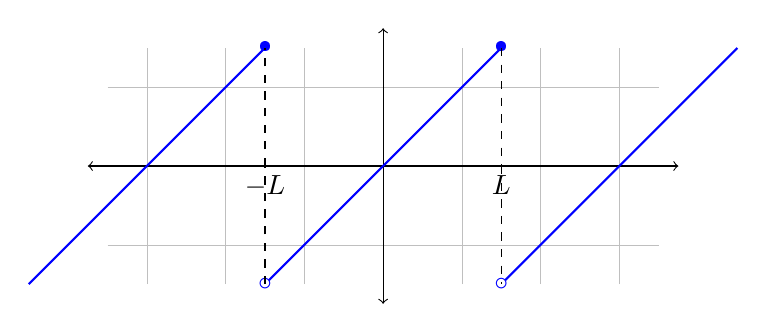
\begin{tikzpicture}
	  \draw[ultra thin,color=lightgray] (-3.5,-1.5) grid (3.5,1.5);   % coordinate grid
	  \draw[<->] (-3.75,0) -- (3.75,0);% node[right] {$x$};   % x-axis
	  \draw[<->] (0,-1.75) -- (0,1.75);% node[above] {$y$};   % y-axis
	
      \draw [thick, samples=100,smooth, color=blue] plot[variable=\t, domain=-4.5:-1.5] ({\t},{\t + 3});
      \draw [thick, samples=100,smooth, color=blue] plot[variable=\t, domain=-1.45:1.5] ({\t},{\t});
      \draw [thick, samples=100,smooth, color=blue] plot[variable=\t, domain=1.55:4.5] ({\t},{\t - 3});

      \node at (-1.5, -1.5) {\color{blue} $\circ$};
	\node at (-1.5, 1.5) {\color{blue} \textbullet};

      \node at (1.5, -1.5) {\color{blue} $\circ$};
	\node at (1.5, 1.5) {\color{blue} \textbullet};

    \draw  [dashed] (1.5, 1.5) -- (1.5, 0) node [below] {$L$};
    \draw [dashed] (1.5, 0) -- (1.5, -1.5);
    \draw  [dashed] (-1.5, -1.5) -- (-1.5, 0) node [below] {$-L$};
    \draw [dashed] (-1.5, 0) -- (-1.5, 1.5);

	\end{tikzpicture}
	\end{center}

    Here we have
    $$
a_n = \frac{1}{L}\int_{-L}^L x \cos \frac{n \pi x}{2} \dd x = 0, \quad \quad \text{(integrating an odd function)}
    $$
    for all $n$, and
    \begin{align*}
        b_n &= \frac{2}{L} \int_0^L x \sin \frac{n \pi x}{L} \dd x   \\
            &= \frac{-2}{n \pi}\left[x \cos \frac{n \pi x}{L}\right]_{0}^{L} + \frac{2}{n \pi} \int_{0}^{h} \cos \frac{n \pi x}{L} \dd x \\
            &= -\frac{2 L}{n \pi} \cos n \pi+\frac{2 L}{(n \pi)^{2}} \cancel{\sin n \pi} \\
            &= \frac{2L}{n \pi} (-1)^{n + 1}.
    \end{align*}
    So the sawtooth Fourier series is 
    $$
    2 L \sum_{n=1}^{\infty} \frac{(-1)^{n+1}}{n \pi} \sin \left(\frac{n \pi x}{L}\right)=\frac{2 L}{\pi}\left[\sin \left(\frac{\pi x}{L}\right)-\frac{1}{2} \sin \left(\frac{2 \pi x}{L}\right)+\frac{1}{3} \sin \left(\frac{3 \pi x}{L}\right) + \cdots\right].
    $$
    which is slowly convergent.

    %L = 1.5
    \begin{center}
    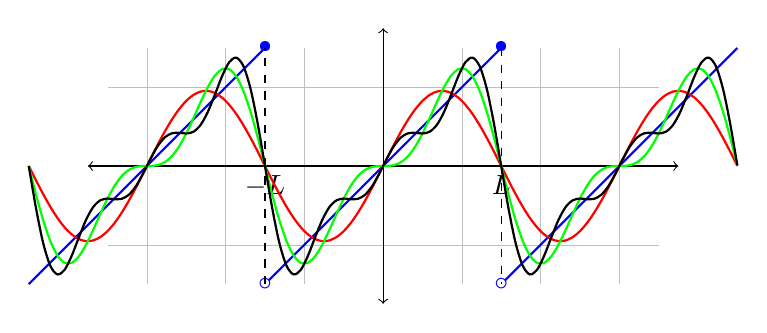
\begin{tikzpicture}
        \draw[ultra thin,color=lightgray] (-3.5,-1.5) grid (3.5,1.5);   % coordinate grid
        \draw[<->] (-3.75,0) -- (3.75,0);% node[right] {$x$};   % x-axis
        \draw[<->] (0,-1.75) -- (0,1.75);% node[above] {$y$};   % y-axis
      
        \draw [thick, samples=100,smooth, color=blue] plot[variable=\t, domain=-4.5:-1.5] ({\t},{\t + 3});
        \draw [thick, samples=100,smooth, color=blue] plot[variable=\t, domain=-1.45:1.5] ({\t},{\t});
        \draw [thick, samples=100,smooth, color=blue] plot[variable=\t, domain=1.55:4.5] ({\t},{\t - 3});
  
        \node at (-1.5, -1.5) {\color{blue} $\circ$};
      \node at (-1.5, 1.5) {\color{blue} \textbullet};
  
        \node at (1.5, -1.5) {\color{blue} $\circ$};
      \node at (1.5, 1.5) {\color{blue} \textbullet};
  
      \draw  [dashed] (1.5, 1.5) -- (1.5, 0) node [below] {$L$};
      \draw [dashed] (1.5, 0) -- (1.5, -1.5);
      \draw  [dashed] (-1.5, -1.5) -- (-1.5, 0) node [below] {$-L$};
      \draw [dashed] (-1.5, 0) -- (-1.5, 1.5);

      % Fourier Series

      \draw [thick, samples=100,smooth, color=red] plot[variable=\t, domain=-4.5:4.5] ({\t},{(2*1.5/pi) * (sin(180 * \t / 1.5))});
      \draw [thick, samples=100,smooth, color=green] plot[variable=\t, domain=-4.5:4.5] ({\t},{(2*1.5/pi) * (sin(180 * \t / 1.5) - 0.5 * sin(2 * 180 * \t / 1.5))});
      \draw [thick, samples=100,smooth, color=black] plot[variable=\t, domain=-4.5:4.5] ({\t},{(2*1.5/pi) * (sin(180 * \t / 1.5) - 0.5 * sin(2 * 180 * \t / 1.5) + (1/3) * sin(3 * 180 * \t / 1.5))});
      
      \end{tikzpicture}
      \end{center}
\end{example}
% \begin{proposition}[Properties of $\sin$ and $\cos$]
    
% \end{proposition}

\subsection{The Dirichlet Conditions (Fourier's Theorem)}

So we need `well behaved' functions for what we have discussed about Fourier series to work, and for a Fourier series for $f$ to be unique. But what exactly does it mean for a function to be `well behaved' in this context?
This is specified by the Dirichlet conditions, also known as Fourier's theorem.

\begin{theorem}[The Dirichlet Conditions]
    If $f$ is a bounded periodic function with period $2L$ and finitely many minima, maxima and discontinuities on $0 \leq x \leq 2L$, then the Fourier series converges to $f(x)$ at all points where $f$ is continuous, and at discontinuities converges to $\frac{1}{2}(f(x_+) + f(x_-))$.
\end{theorem}

One might note that these conditions are \emph{much weaker} than those needed for Taylor series, but it does eliminate pathological functions such as $\sin 1/x$, $1/x$ and the indicator function on the rationals. 
The converse of this is \emph{not} true, for example $\sin 1/x$ has a well defined Fourier series. 

The proof of this result is \emph{too} difficult, but is best done using complex methods so we will not dwell on it in this course.

The rate of convergence of the Fourier series depends on the `smoothness' of the function.

\begin{theorem}[Rate of Convergence of Fourier Series]
If $f(x)$ has continuous derivatives up to a $p$th derivative which is discontinuous, then the Fourier series converges as $\mathcal{O}(n^{-(p + 1)})$ as $n \rightarrow \infty$.    
\end{theorem}

\begin{example}[Square Wave]\label{ex:square}
    Consider the function
    $$
    f(x) \begin{cases}
        1 &\mbox{if } 0 \leq x < 1, \\
        -1 &\mbox{if } -1 \leq x < 0.
       \end{cases}
    $$
    This function has discontinuous $p = 0$th derivative (the function is discontinuous!), and the fourier series of this function is given by
    $$
    f(x) = 4 \sum_{m=1}^{\infty} \frac{\sin (2 m-1) \pi x}{(2 m-1) \pi}.
    $$
\end{example}

\begin{example}[`See-Saw' Wave]
    Consider the function
    $$
    f(x) \begin{cases}
        x(1 - \xi) &\mbox{if } 0 \leq x < \xi, \\
        \xi(1 - x) &\mbox{if } \xi \leq x < 1,\\
        f(-x) &\mbox{if } -1 \leq x < 0.
       \end{cases}
    $$
    This function has discontinuous $p = 1$st derivative, and it's Fourier series is given by
    $$
       f(x) = 2 \sum_{m=1}^{\infty} \frac{\sin (n \pi \xi) \sin (n \pi x)}{(n \pi)^{2}}.
    $$
\end{example}

\subsubsection*{Integration of Fourier Series}

As a general principle, it is \emph{always} valid to integrate the Fourier series of $f(x)$ term-wise to obtain
$$
F(x) = \int_{-x}^x f(x) \dd x,
$$
because $F(x)$ satisfies the Dirichlet conditions if $f(x)$ does. 

\subsubsection*{Differentiation of Fourier Series}

As a general principle, you must \emph{take care} when differentiating a Fourier series term-wise. Let's look at an example.

\begin{example}[Differentiating the Square Wave]
    Consider the clearly non-differentiable square wave function, defined in \autoref{ex:square}. We had
    $$
    f(x)=4 \sum_{m=1}^{\infty} \frac{\sin (2 m-1) \pi x}{(2 m-1) \pi}.
    $$
    We can try and differentiate this term-wise to get
    $$
    f^{\prime}(x) \stackrel{?}{=} 4 \sum_{m=1}^{\infty} \cos (2 m-1) \pi x,
    $$
    but this series is unbounded!
\end{example}

So we need to be careful. Here's the result about what we can do with differentiation.

\begin{theorem}
    If $f(x)$ is continuous and satisfies the Dirichlet conditions, and $f'(x)$ satisfies the Dirichlet conditions, then $f'(x)$ can be found by term-wise differentiation of the Fourier series of $f(x)$.
\end{theorem}

\subsection{Parseval's Theorem}

Parseval's theorem is a relation between the integral of the square of a function and the square of the Fourier coefficients:

\begin{align*}
    \int_{0}^{2L}[f(x)]^{2} \dd x&=\int_{0}^{2 L} \dd x\left[\frac{1}{2} a_{0}+\sum_{n} a_{k} \cos \frac{n \pi x}{L}+\sum_{n} b_{n} \sin \frac{n \pi x}{L}\right]^{2} \\ 
&= \int_{0}^{2 L} \dd x\left[\frac{1}{4} a_{0}^{2}+\sum_{n} a_{n}^{2} \cos ^{2} \frac{n \pi x}{L}+\sum_{n} b_{n}^{2} \sin ^{2} \frac{n \pi x}{L}\right] \\
&= 2\left[\frac{1}{2} a_{0}^{2}+\sum_{n=1}^{\infty}\left(a_{n}^{2}+b_{n}^{2}\right)\right].
\end{align*}

This result is also called the completeness relation, since the $LHS \geq RHS$ if any of the basis functions are missing.

\begin{example}[The Basel Problem]
    Consider the sawtooth wave $f(x) = x$ on $-L \leq x \leq L$. The the LHS is
    $$
    \int_{-L}^{L} x^2 \dd x = \frac{2}{3}L^3,
    $$
    and the RHS is
    $$
    L \sum_{n = 1}^{\infty} \frac{4L^2}{n^2 \pi^2} = \frac{4L^3}{\pi^2}\sum_{n = 1}^{\infty} \frac{1}{n^2},
    $$
    and thus $\sum_{n = 1}^{\infty} 1/n^2 = \pi^2/6$.
\end{example}


\subsection{Alternative Fourier Series}

There are some alternative forms of fourier series.

\subsubsection*{Half-Range Series}

Consider $f(x)$ defined only on $0 \leq x < L$. We can extend it's range over $-L \leq x < L$ in two simple ways:
\begin{enumerate}
    \item Require $f$ to be odd, with $f(-x) = -f(x)$. Then considering it's Fourier series we would have $a_n = 0$ for all $n$ (as $\cos$ is even), and
    $$
    b_{n}=\frac{2}{L} \int_{0}^{L} f(x) \sin \frac{n \pi x}{2} \dd x.
    $$
    This implies that $f(x) = \sum_{n= 1}^{\infty} b_n \sin \frac{n \pi x}{L}$, which is a \vocab{Fourier sine series}.
    \item Require $f$ to be even, with $f(-x) = f(x)$, Then $b_n = 0$, and
    $$
    a_{n}=\frac{2}{L} \int_{0}^{2} f(x) \cos \frac{n \pi x}{L} \dd x,
    $$
    so $f(x) = \frac{1}{2}a_0 + \sum_{n = 1}^{\infty} a_n \cos\frac{n \pi x}{L}$, which is a \vocab{Fourier cosine series}.
\end{enumerate}

\subsubsection*{Complex Representation}

Recall that we can write
$$
\cos \frac{n \pi x}{L} = \frac{1}{2}\left(e^{in \pi x/L} + e^{-i n \pi x/L}\right) \quad \text{and} \quad \sin \frac{n \pi x}{L} = \frac{1}{2i} \left(e^{i n \pi x/L} - e^{-i n \pi x/L} \right).
$$
So the Fourier series is
\begin{align*}
    f(x) &= \frac{1}{2} a_{0}+\sum_{n=1}^{\infty} a_{n} \cos \frac{n \pi x}{L}+\sum_{n=1}^{\infty} b_{n} \sin \frac{n \pi x}{2} \\
    &= \frac{1}{2} a_{0}+\sum_{n=1}^{\infty}\left(a_{n}-i b_{n}\right) e^{i n \pi x / L}+\sum_{n=1}^{\infty}\left(a_{n}+i b_{n}\right) e^{-i n \pi  x / L} \\
    &= \sum_{m=-\infty}^{\infty} c_{m} e^{i m \pi x / L},
\end{align*}
where for $m > 0$, $c_m = \frac{1}{2}(a_m - i b_m)$ and for $m < 0$, $c_m = \frac{1}{2}(a_{-m} + i b_{-m})$. Equivalently,
$$
c_m = \frac{1}{2L} \int_{-L}^L f(x) e^{-i m \pi x/L } \dd x.
$$

\subsection{Some Fourier Series Motivations -- Self-Adjoint Matrices}

We will now review a few results about matrices. Suppose that $\vv u, \vv v \in \C^n$ with inner product $\langle \vv u, \vv v\rangle = \vv u^\dagger \vv v$.
The $n \times n$ matrix $A$ is \vocab{self-adjoint} or \vocab{hermitian} if
$$
\langle A \vv u, v\rangle = \langle u, A \vv v\rangle,
$$
that is, if $A^\dagger = A$.

The eigenvalues $\lambda_i$ and eigenvectors $\vv v_i$ satisfy
$$
A \vv v_i = \lambda_i \vv v_i,
$$
and have the following properties
\begin{enumerate}[label=(\roman*)]
    \item The eigenvalues are real
    \item If $\lambda_i \neq \lambda_j$, then the corresponding eigenvectors are orthogonal with $\langle \vv v_i, \vv v_j\rangle = 0$
    \item We can rescale to create an orthonormal basis $\{\vv v_1, \dots, \vv v_n\}$.
\end{enumerate}

Given $\vv b$, we can solve for $\vv x$ in the equation
$$
A \vv x = \vv b.
$$
Express $\vv b = \sum_{i = 1}^n b_i \vv v_i$, and we seek a solution $\vv x = \sum_{i = 1}^n c_n \vv v_n$. Substituting this into the above equation, we get
$$
A \vv x = \sum_{i} A c_i \vv  v_i = \sum_{i} c_i \lambda_i \vv v_i = \sum_{i} b_i \vv v_i.
$$
By orthogonality, we can equate coefficients to get $c_n \lambda_n = b_n$, so our solution is
$$
\vv x = \sum_{i = 1}^n \frac{b_i}{\lambda_i} \vv v_i.
$$

So once we have a self-adjoint matrix $A$ and have found all of the eigenvalues, we then have a general methodology for solving any matrix equation of the form $A \vv x = \vv b$. It turns out that you can do the same with Fourier series!

We can find a general solution to the differential equation for which cosines and sines are the eigenfunctions.

\subsection{Solving Inhomogeneous ODEs with Fourier Series}

We wish to find $y(x)$ given $f(x)$ for the differential operator
$$
\mathcal{L}[y] \equiv -\frac{\dd^2 y}{\dd x^2} = f(x).
$$
To solve this, we need some boundary conditions, which we will take as $y(0) = y(L) = 0$.

The related eigenvalue problem is
$$
\mathcal{L}[y_n] = \lambda_n y_n,
$$
with $y_n(0) = y_n(L) = 0$, which has eigenfunctions and eigenvalues
$$
y_n(x) = \sin \frac{n \pi x}{L}, \quad \lambda_n = \left(\frac{n \pi }{L}\right)^2.
$$

We seek solutions as half-range sine series. To do that, we will try substitute $y(x) = \sum_{n = 1}^{\infty} c_n \sin \frac{n \pi x}{L}$, and expand $f(x)$ in terms of it's fourier series, $f(x) = \sum_{n = 1}^{\infty} b_n \sin \frac{n \pi x}{L}$, with $b_n = \frac{2}{L} \int_0^L f(x) \sin \frac{n \pi x}{L} \dd x$.

Substituting this into the differential equation, we get
$$
\mathcal{L}[y] = - \frac{\dd^2}{\dd x^2} \left(\sum_{n = 1}^{\infty} c_n \sin \frac{n \pi x}{L}\right) = \sum_{n = 1}^{\infty} c_n \left(\frac{n \pi}{L}\right)^2 \sin \frac{n \pi x}{L}.
$$
By orthogonality, we have $c_n \left(\frac{n \pi }{L}\right)^2 = b_n$, so the solution is
$$
y(x) = \sum_{n = 1}^{\infty} \frac{b_n}{\left(\frac{n \pi }{L}\right)^2}\sin \frac{n \pi x}{L} = \sum_{n = 1}^{\infty} \frac{b_n}{\lambda_n} y_n.
$$

\begin{example}
    Consider the `square wave' source given by $f(x) = 1$ for $0 \leq x < 1$, with the function being odd. This function has fourier series
    $$
    f(x)=4 \sum_{m=1}^{\infty} \frac{\sin (2 m-1) \pi x}{(2 m-1) \pi}.
    $$
    So the solution for $y$ must then by
    $$
    y(x)=\sum_{n} \frac{b_{n}}{\lambda_{n}} y_{n}=4 \sum_{m} \frac{\sin (2 m-1) \pi x}{((2 m-1) \pi)^{3}},
    $$
    but this is the Fourier series for $y(x) = \frac{1}{2}x(1 - x)$!
\end{example}

\end{document}
